\documentclass{article}
\usepackage[utf8]{inputenc}
\usepackage{multicol}
\usepackage{geometry}
\usepackage{multirow}
\usepackage{booktabs}
\setlength{\columnsep}{30pt} 
\usepackage{frontespizio}
\usepackage[T1]{fontenc}
\usepackage[utf8]{inputenc}
\usepackage{amsfonts}
\usepackage{amsmath}
\usepackage{bm}
\usepackage{empheq}
\usepackage{csquotes}
\usepackage[backend=biber,sorting=none]{biblatex} 
\usepackage{lipsum}
\usepackage{listings}
\usepackage[font=small,labelfont=bf]{caption}
\usepackage{url}
\usepackage[table]{xcolor}
\usepackage{float}
\usepackage[section]{placeins}
 \graphicspath{ {./Figures/} }
\usepackage{graphicx,subfig,caption}
\usepackage{subfig}
\addbibresource{bibliography.bib}  

 \usepackage{nicematrix}
\definecolor{codegreen}{rgb}{0,0.6,0}
\definecolor{codegray}{rgb}{0.5,0.5,0.5}
\definecolor{codepurple}{rgb}{0.58,0,0.82}
\definecolor{backcolour}{rgb}{0.95,0.95,0.92}







\geometry{margin=2cm}

\lstdefinestyle{mystyle}{
backgroundcolor=\color{backcolour},
commentstyle=\color{codegreen},
keywordstyle=\color{magenta},
numberstyle=\tiny\color{codegray},
stringstyle=\color{codepurple},
basicstyle=\ttfamily\footnotesize,
breakatwhitespace=true,
breaklines=true,
captionpos=b,
keepspaces=true,
numbers=left,
numbersep=8pt,
showspaces=false,
showstringspaces=false,
showtabs=false,
tabsize=2,
breakindent=0pt ,
columns=fullflexible,
postbreak=\mbox{\textcolor{red}{$\hookrightarrow$}\space}
}



\lstset{breaklines=true}


\begin{document}


\title{LSTM autoencoder for anomaly detection on ECG data}
\author{R. Lorusso, A. Urso}
\date{2023 - University of Bari Aldo Moro}

\maketitle

\begin{multicols*}{2}

\section*{Abstract}
\begin{it}
The aim of this work is to provide a model for effectively identify anomalies in ECGs. The proposed approach is that of an LSTM autoencoder which can both capture the sequential nature of such data and discriminate the anomaly based on their reconstruction error.

\end{it}



\section{Introduction}

The detection of anomalies, also known as outliers, is an integral practice across a diverse range of disciplines. Anomalies can indicate a breach of a system or network, signal abnormal physiological levels, or even flag the occurrence of fraud. Regardless of the particular application, analytics and machine learning models have the potential to provide both predictive and descriptive value. Anomaly detection can be used to inform about anomalous data that can be indicative of health complications. This kind of information can be very useful to professionals as a first insight to a possible patient problem. Since providing care and track patient vitals signals can be hard to maintain trough the time, machine learning can be very helpful by automatically detect rare deviations from normal data trends, thus providing health care professionals with useful information with which make more accurate and quicker clinical decisions. However what is to be considered as an anomaly isn't ever clearly defined. The main assumptions are that anomalies are infrequent an somehow they differ from normal data. Furthermore anomalies can differ substantially one from each other, thus introducing more uncertainty about their nature. Sometimes oscillations in the test data can be detected as anomalies, introducing false alarms. Especially in the e-health domain, we are interested in reducing or minimizing the number of false alerts, since an high false alarm rate can decrease the trust in the system and in the alarm itself.
We'll proceed by describing the dataset, the preprocessing strategy and then we will move to focus on the employed model, describing its architecture and the motivations behind it. Finally we'll analyze related works and the final results obtained from the experiments. 

\section{Dataset Description}

 The dataset is called “ECG5000” which is a 20-hour long ECG downloaded from Physionet. As the name suggests, it is composed by 5000 ECG traces and it was originally published in “Goldberger AL, Amaral LAN, Glass L, Hausdorff JM, Ivanov PCh, Mark RG, Mietus JE, Moody GB, Peng C-K, Stanley HE. PhysioBank, PhysioToolkit, and PhysioNet: Components of a New Research Resource for Complex Physiologic Signals. Circulation 101(23)”.
 

\section{Employed model}

Since we are dealing with sequential data, we chose to use an LSTM autoencoder to catch the temporal nature of the ECG, while learning a latent representation of it. The aim is to detect an anomaly by evaluating the reconstruction error between the input and the output of the autoencoder. By encoding the input, the neural network learns the most important features in the data and, after the decoding, we can compare the input to the output and examine the difference. If there is a big difference (the reconstruction loss is high) then we can assume that the model struggled in reconstructing the data, thus this data point is suspected as an anomaly.

\begin{figure}[H]
  \centering
  \subfloat[Autoencoder]{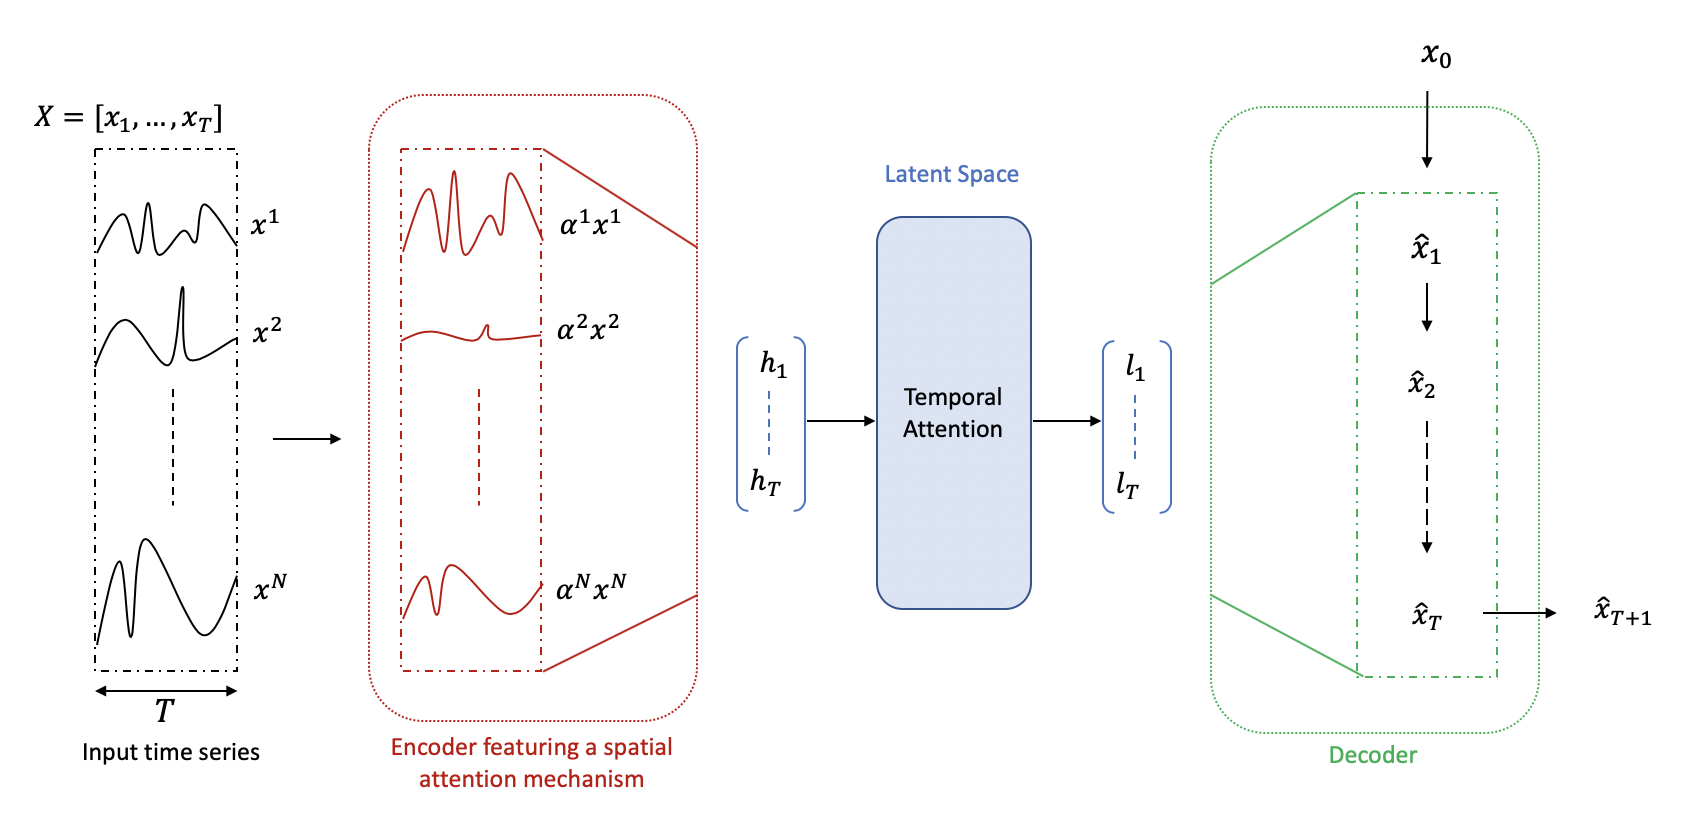
\includegraphics[width=\linewidth]{images/autoencoder.png}\label{fig:f1}}
\end{figure}


\section{Feature Engineering }

\section{Model development}


\subsection{Parameter Tuning} 


\subsection{Ground Truth} 


\subsection{Training and Validation Data} 


\subsection{Testing Data} 



\section{Related Works}



\section{Experimental results}
\label{'Results'}



\nocite{*}



\end{multicols*}

\end{document}





